% Taller 6 -- Series de tiempo. Compilar:
% tectonic -Z search-path=$HOME/repos/ud/maestria/mcic/.UniversidadDistrital-manual-marca/plantillas-latex informe_taller6.tex
% Las cifras salen de taller6_series_tiempo.ipynb ejecutado; las figuras, de ../figuras/.
\documentclass[11pt,letterpaper]{article}
\usepackage{ud-informe}
\usepackage{amsmath}
\colorlet{udrojo}{udazul}
\definecolor{udrojoosc}{HTML}{0C6F96}

\renewcommand{\UDtitulo}{Modelo clásico frente a redes NAR y NARX}
\renewcommand{\UDsubtitulo}{Pronóstico de PM2.5 diario en Beijing con validación de origen móvil y prueba de Diebold-Mariano}
\renewcommand{\UDtipo}{Taller 6 -- Informe}
\renewcommand{\UDasignatura}{Inteligencia Computacional Aplicada}
\renewcommand{\UDdocente}{Cesar Andrey Perdomo Charry}
\renewcommand{\UDestudiantes}{Juan Felipe Rodríguez Galindo -- 20261595004}
\renewcommand{\UDencabezado}{Taller 6 -- Series de tiempo}

\begin{document}
\UDportada

\section{Introducción}

El objetivo del taller es comparar un modelo estadístico clásico con una red neuronal autorregresiva no lineal sobre una serie real, y decidir con evidencia estadística si la red pronostica mejor. Usé la plantilla del curso, \textit{TallerST\_Plantilla.ipynb}, que ya trae la carga, la validación del conjunto, el diagnóstico, la validación cruzada de origen móvil, las métricas, el análisis de residuos y la prueba de Diebold-Mariano. Resolví sus tres \texttt{TODO-EQUIPO}: \texttt{modelo\_clasico}, \texttt{modelo\_neuronal} y \texttt{REJILLAS}. No modifiqué el motor de evaluación y ejecuté la prueba externa una sola vez, al final. Desarrollé solo la versión en Python; la versión en MATLAB no la hice porque no tengo MATLAB.

Elegí el conjunto \textit{Beijing Multi-Site Air Quality} (UCI), estación Aotizhongxin: la contaminación por partículas finas PM2.5 se relaciona físicamente con el clima (el viento la dispersa), que es el escenario en que una NARX con variables exógenas debería aportar. Entregables: el cuaderno \texttt{taller6\_series\_tiempo.ipynb} ejecutado con sus salidas, la carpeta \texttt{resultados/}, \texttt{requirements.txt} y este informe.

\section{Marco teórico}

\textbf{Estacionariedad y estacionalidad.} La prueba ADF tiene como hipótesis nula una raíz unitaria y la KPSS, estacionariedad; usarlas juntas evita decidir con una sola. La descomposición STL separa tendencia, estacionalidad y residuo, y la fuerza estacional $F_S = \max\{0,\, 1-\operatorname{Var}(R)/\operatorname{Var}(S+R)\}$ mide qué tan marcado es el ciclo, con $s$ el número de pasos de un periodo (aquí $s=7$ días).

\textbf{SARIMAX.} Un modelo $\mathrm{SARIMAX}(p,d,q)(P,D,Q)_s$ combina una parte autorregresiva de orden $p$, $d$ diferencias, una media móvil de orden $q$, sus análogos estacionales y regresores exógenos lineales $\beta^\top x_t$. El orden se elige con los criterios de información
\begin{equation*}
\mathrm{AIC} = 2k - 2\ln L, \qquad \mathrm{BIC} = k\ln n - 2\ln L,
\end{equation*}
que premian la verosimilitud $L$ y castigan los $k$ parámetros (BIC con más fuerza). La prueba de Ljung-Box verifica si a los residuos les queda autocorrelación.

\textbf{NAR y NARX.} Una red NAR aproxima $y_t = f(y_{t-1},\dots,y_{t-d_y}) + \varepsilon_t$ con un perceptrón multicapa; la NARX agrega las exógenas, $f(y_{t-1},\dots,y_{t-d_y},\, x_t,\dots,x_{t-d_x})$. Se entrena en \textbf{lazo abierto}, con los retardos reales como entradas, y pronostica en \textbf{lazo cerrado}: cada pronóstico vuelve como retardo del paso siguiente, por lo que el error puede acumularse con el horizonte.

\textbf{Evaluación.} Con errores $e_t = y_t - \hat y_t$, se usan $\mathrm{RMSE}=\sqrt{\overline{e^2}}$, $\mathrm{MAE}=\overline{|e|}$ y el error absoluto escalado $\mathrm{MASE} = \mathrm{MAE}/\mathrm{MAE}_{\text{ingenuo}}$, donde el denominador es el error del ingenuo estacional $\hat y_t = y_{t-s}$ en el desarrollo; $\mathrm{MASE}<1$ indica un modelo mejor que repetir la semana anterior. La prueba de Diebold-Mariano contrasta $H_0: \mathrm{E}[d_t]=0$ con $d_t = e_{1,t}^2 - e_{2,t}^2$, con la varianza corregida por la autocorrelación hasta el horizonte $h$ y el ajuste de Harvey, Leybourne y Newbold para muestras pequeñas.

\section{Metodología}

\textbf{Datos.} La plantilla promedia por día los registros horarios de marzo de 2013 a febrero de 2017 (1461 días) y rellena por interpolación temporal los 15 días sin PM2.5. La serie objetivo es PM2.5 en $\mu$g/m$^3$ y las exógenas son temperatura (TEMP), punto de rocío (DEWP), presión (PRES) y velocidad del viento (WSPM). Cumple los criterios C1 a C6 de la plantilla. La partición es temporal: 1168 días de desarrollo (80\,\%) y 293 de prueba externa (20\,\%). Como en el taller resuelto en clase, el clima de los días a pronosticar se toma como conocido.

\textbf{Validación.} El motor usa origen móvil con ventana expandible: 5 orígenes repartidos en el último 40\,\% del desarrollo y horizonte $H=24$ días; cada pliegue entrena con todo lo anterior a su origen. La prueba externa usa 12 orígenes sobre los 293 días finales. Todos los modelos cumplen el mismo contrato \texttt{pronosticar(y\_hist, X\_hist, X\_fut, H, **hp)} y todo lo que depende de los datos se ajusta dentro de cada llamada, solo con \texttt{y\_hist} y \texttt{X\_hist}.

\textbf{Modelo clásico.} PM2.5 es positiva y muy asimétrica (asimetría 1,77 en el desarrollo), así que modelé $z_t=\log(1+y_t)$, que la reduce a $-0{,}28$, y devolví $\exp(\hat z)-1$. Las pruebas ADF y KPSS indicaron una serie estacionaria en nivel ($d=0$) y la STL una estacionalidad semanal débil ($F_S = 0{,}07$). Comparé con AIC y BIC los órdenes $p,q\in\{0,1,2\}$ con y sin término estacional $(1,0,1)_7$, con constante y las cuatro exógenas.

\textbf{Red neuronal.} Implementé una NARX en Keras: entradas $y_{t-1},\dots,y_{t-d_y}$ y las cuatro exógenas en $t$, $t-1$ y $t-2$ ($d_x = 2$); una capa oculta \texttt{tanh} con regularización L2 ($10^{-4}$) y una salida lineal; Adam con tasa $10^{-3}$, lotes de 32 y hasta 300 épocas con parada temprana (paciencia 20, con los mejores pesos) sobre el 15\,\% final de la historia. La serie se transforma con $\log(1+y)$ y se estandariza con la media y la desviación de \texttt{y\_hist}; las exógenas, con las de \texttt{X\_hist}. La NAR es la misma función sin exógenas.

\textbf{Sensibilidad.} La rejilla del clásico recorre $p\in\{1,2,3\}\times q\in\{0,1,2\}$; la de la red, $d_y\in\{7,14,28\}\times$ neuronas $\in\{5,10,20\}\times$ semilla $\in\{1,2,3\}$, es decir 27 configuraciones y 135 entrenamientos. Para la red promedié el RMSE de validación sobre las tres semillas y elegí la combinación de menor media. Los hiperparámetros se eligieron solo con la validación cruzada, antes de mirar la prueba externa.

\section{Resultados}

\subsection{Identificación del clásico}

La tabla~\ref{tab:aic} resume los mejores órdenes. AIC y BIC eligen el mismo modelo, ARIMAX$(1,0,1)$ sin parte estacional, coherente con $F_S=0{,}07$.

\begin{table}[H]
\centering
\caption{Mejores órdenes según AIC sobre el desarrollo (con constante y exógenas, $s=7$).}\label{tab:aic}
\begin{tabular}{llcc}
\toprule
Orden & Estacional & AIC & BIC \\
\midrule
$(1,0,1)$ & $(0,0,0)_7$ & \textbf{1991,2} & \textbf{2031,7} \\
$(1,0,2)$ & $(0,0,0)_7$ & 2003,7 & 2049,3 \\
$(1,0,2)$ & $(1,0,1)_7$ & 2006,4 & 2062,1 \\
\bottomrule
\end{tabular}
\end{table}

Los coeficientes del modelo elegido tienen el signo esperado: el punto de rocío sube la contaminación ($+0{,}110$, con $p<0{,}001$), mientras el viento ($-0{,}123$) y la temperatura ($-0{,}061$) la bajan; la presión no resulta significativa ($p=0{,}58$). La parte ARMA es $\phi_1=0{,}854$ y $\theta_1=-0{,}352$. Aun así, Ljung-Box rechaza la ausencia de autocorrelación en los residuos en los rezagos 7, 14 y 21: queda estructura que un modelo lineal no captura.

\subsection{Validación cruzada}

La tabla~\ref{tab:cv} compara los modelos en los 5 pliegues, con los hiperparámetros iniciales ($p=q=1$; $d_y=14$ y 10 neuronas) y con los elegidos por la rejilla.

\begin{table}[H]
\centering
\caption{Validación cruzada de origen móvil (5 pliegues, $H=24$). RMSE y MAE en $\mu$g/m$^3$.}\label{tab:cv}
\begin{tabular}{lcccc}
\toprule
& \multicolumn{2}{c}{Iniciales} & \multicolumn{2}{c}{Elegidos} \\
\cmidrule(lr){2-3}\cmidrule(lr){4-5}
Modelo & RMSE & MASE & RMSE & MASE \\
\midrule
Ingenuo estacional & 110,53 & 1,005 & 110,53 & 1,005 \\
Clásico (ARIMAX) & 52,50 & 0,521 & 52,50 & 0,521 \\
NARX & 43,33 & 0,421 & 42,81 & 0,446 \\
NAR & 59,75 & 0,608 & 61,38 & 0,622 \\
\bottomrule
\end{tabular}
\end{table}

\subsection{Sensibilidad}

En el clásico, el mejor orden de la rejilla vuelve a ser $p=1$, $q=1$ (RMSE medio 50,66), el mismo que eligieron AIC y BIC. En la red (figura~\ref{fig:sens}), la mejor combinación es $d_y=7$ con 20 neuronas: RMSE medio de 38,80 con desviación de 0,20 entre semillas. El factor que más mueve el error son los retardos: con $d_y=28$ el RMSE sube a entre 45 y 50, mientras que con $d_y$ fijo cambiar el número de neuronas lo mueve entre 1 y 5 puntos. La semilla también pesa: con $d_y=28$ y 5 neuronas la desviación entre semillas llega a 7 puntos, lo que justifica promediar.

\begin{figure}[H]
\centering
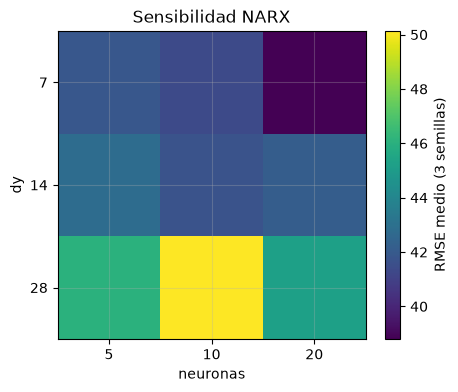
\includegraphics[width=0.48\linewidth]{../figuras/sensibilidad_narx.png}
\caption{RMSE medio de validación de la NARX (3 semillas) según retardos $d_y$ y neuronas.}\label{fig:sens}
\end{figure}

\subsection{Prueba externa}

Con los hiperparámetros elegidos ($p=q=1$; $d_y=7$, 20 neuronas), la prueba externa se ejecutó una sola vez (tabla~\ref{tab:test}, figuras~\ref{fig:horiz} y~\ref{fig:pron}).

\begin{table}[H]
\centering
\caption{Prueba externa: 12 orígenes, $H=24$. Tiempo total de ajuste y pronóstico.}\label{tab:test}
\begin{tabular}{lcccc}
\toprule
Modelo & RMSE & MAE & MASE & Tiempo (s) \\
\midrule
Ingenuo estacional & 96,24 & 69,49 & 0,974 & 0,0 \\
Clásico (ARIMAX) & 68,47 & 43,55 & 0,610 & 6,3 \\
NARX & \textbf{49,61} & \textbf{29,33} & \textbf{0,411} & 62,4 \\
NAR & 76,04 & 48,30 & 0,677 & 39,7 \\
\bottomrule
\end{tabular}
\end{table}

\begin{figure}[H]
\centering
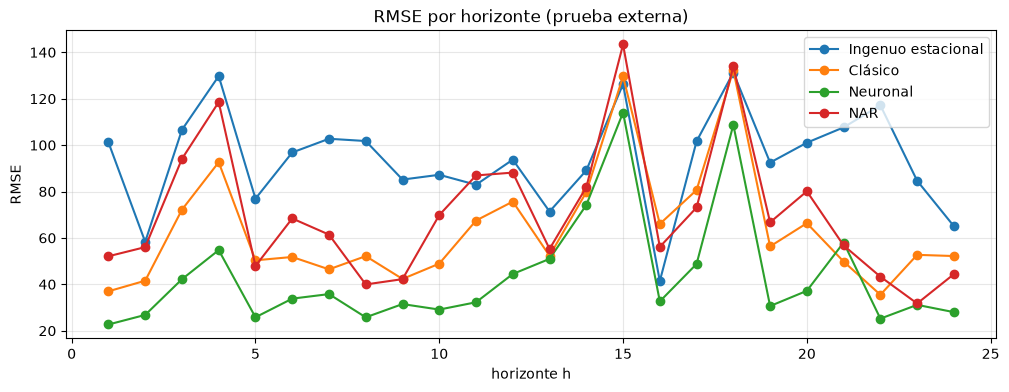
\includegraphics[width=0.7\linewidth]{../figuras/rmse_horizonte.png}
\caption{RMSE por horizonte en la prueba externa.}\label{fig:horiz}
\end{figure}

\begin{figure}[H]
\centering
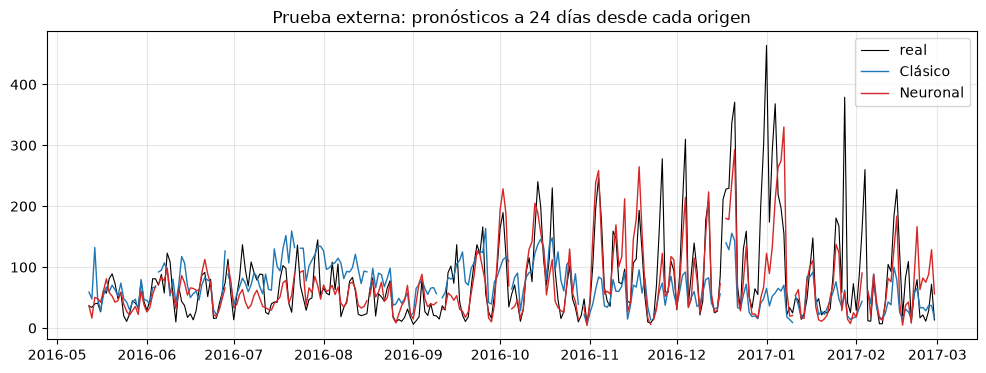
\includegraphics[width=\linewidth]{../figuras/pronosticos_prueba.png}
\caption{Prueba externa: serie real y pronósticos a 24 días desde cada origen del clásico y la NARX.}\label{fig:pron}
\end{figure}

\subsection{Residuos y Diebold-Mariano}

Ljung-Box rechaza la ausencia de autocorrelación en los residuos de todos los modelos: ninguno extrae toda la estructura de la serie, algo esperable al pronosticar 24 días con errores que se encadenan. La tabla~\ref{tab:dm} resume la prueba de Diebold-Mariano sobre la prueba externa.

\begin{table}[H]
\centering
\caption{Diebold-Mariano con corrección HLN ($h=24$, pérdida cuadrática). Un estadístico positivo indica que el segundo modelo tiene menor error.}\label{tab:dm}
\begin{tabular}{lcc}
\toprule
Comparación & DM$^*$ & $p$ \\
\midrule
Ingenuo frente a clásico & 2,608 & 0,010 \\
Ingenuo frente a NARX & 2,807 & 0,005 \\
Ingenuo frente a NAR & 2,340 & 0,020 \\
Clásico frente a NARX & 2,246 & \textbf{0,026} \\
Clásico frente a NAR & $-1{,}357$ & 0,176 \\
NARX frente a NAR & $-1{,}943$ & 0,053 \\
\bottomrule
\end{tabular}
\end{table}

\section{Análisis}

\textbf{La NARX gana, y la diferencia es significativa.} En la prueba externa la NARX reduce el MASE de 0,610 a 0,411 frente al clásico y Diebold-Mariano rechaza la igualdad ($p=0{,}026$). La NARX tiene el menor RMSE en casi todos los horizontes, con la mayor ventaja en los primeros 12 días; en los horizontes 13 a 15 y 18 los cuatro modelos se acercan, porque ahí caen los picos que ninguno anticipa (figura~\ref{fig:horiz}). Con solo 12 orígenes la curva es irregular y no crece de forma monótona con $h$. En la figura~\ref{fig:pron} se ve dónde gana: entre noviembre y enero el clásico se queda muy por debajo de los episodios de smog, mientras la NARX, que recibe el clima de esos días, sube con ellos.

\textbf{Buena parte de la ventaja viene del clima.} Sin exógenas, la NAR (0,677) queda peor que el clásico, que sí usa el clima, y la diferencia entre NARX y NAR roza la significancia ($p=0{,}053$). La conclusión depende del supuesto de clima futuro conocido: con un pronóstico meteorológico real, con error, la ventaja de la NARX y del ARIMAX sería menor.

\textbf{Más memoria no es mejor.} Con 28 días de retardos la red tiene más entradas que información útil: el error de validación sube de cerca de 40 a entre 45 y 50. Una semana basta, coherente con la memoria corta que sugiere el $\phi_1=0{,}854$ del ARIMAX.

\textbf{La validación anticipó la prueba.} El orden de los modelos en validación (NARX, clásico, NAR, ingenuo) se mantuvo en la prueba externa. El ingenuo incluso mejora en la prueba (MASE 0,974 frente a 1,005), mientras el clásico y la NAR empeoran más que la NARX al pasar de validación a prueba.

\textbf{Costo e interpretabilidad.} La red tarda casi 10 veces más que el clásico en la prueba (62 s frente a 6 s) y sus pesos no se interpretan; el ARIMAX, en cambio, cuantifica el efecto de cada variable del clima. Es un intercambio: precisión con la NARX, explicación con el clásico.

\section{Conclusiones}

\begin{enumerate}
\item PM2.5 diario en Beijing es estacionaria en nivel, con estacionalidad semanal débil ($F_S=0{,}07$); el logaritmo reduce su asimetría de 1,77 a $-0{,}28$.
\item AIC, BIC y la rejilla de validación coinciden en el mismo clásico, ARIMAX$(1,0,1)$ con clima: el punto de rocío aumenta la contaminación y el viento la reduce.
\item En la red pesan más los retardos que las neuronas: una semana de retardos ($d_y=7$) y 20 neuronas dio el menor error medio entre semillas (RMSE 38,80, desviación 0,20).
\item En la prueba externa la NARX supera al clásico (MASE 0,411 frente a 0,610) y la diferencia es significativa ($p=0{,}026$); sin clima, la NAR no supera al clásico.
\item La ventaja de la NARX depende del clima futuro conocido y cuesta casi 10 veces más tiempo de cómputo, con menos interpretabilidad que el ARIMAX.
\end{enumerate}

\end{document}
